\section{Modeling of pressure cell}
\label{section:presure_cell_electic_circuit}

The main focus of the section is to describe the design pressure cell, which is the main measurement component for multiaxial force sensor.
As mentioned in the section on \nameref{section:optical_modeling}, I used the pressure cell design described in the study \cite{my_love_pressure_photosensor} as a guide. 
I selected the photomicrosensor (OMRON EE-SX1321) as the optopair, similar to the authors, because it includes one LED and two phototransistors, 
eliminating the need for separate design and calibration of a reference phototransistor subcircuit. 
This step is important for optocoupler pressure sensor types to ensure that the reference and measurement phototransistors behave identically and any changes in optocoupler characteristics are minimized.

The section describes the electrical circuit and optical barrier designs.

\subsection{Electric circuit design}
% \begin{figure}[H]
%   \centering
%   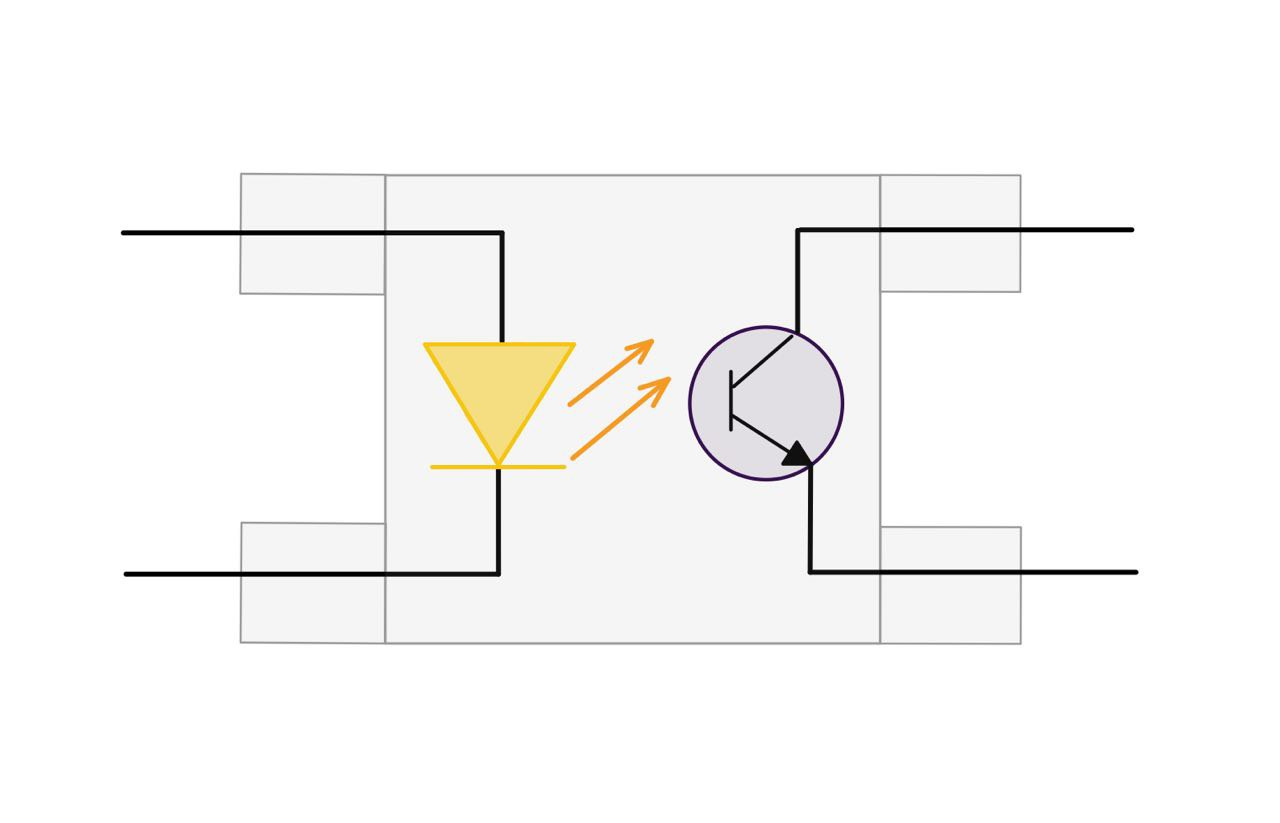
\includegraphics[width=\textwidth]{ED/optopair_scheme.jpg}
%   \label{fig:optopair_scheme}
%   \caption{General design of an optopair.}
% \end{figure}

\begin{figure}[H]
    \centering
    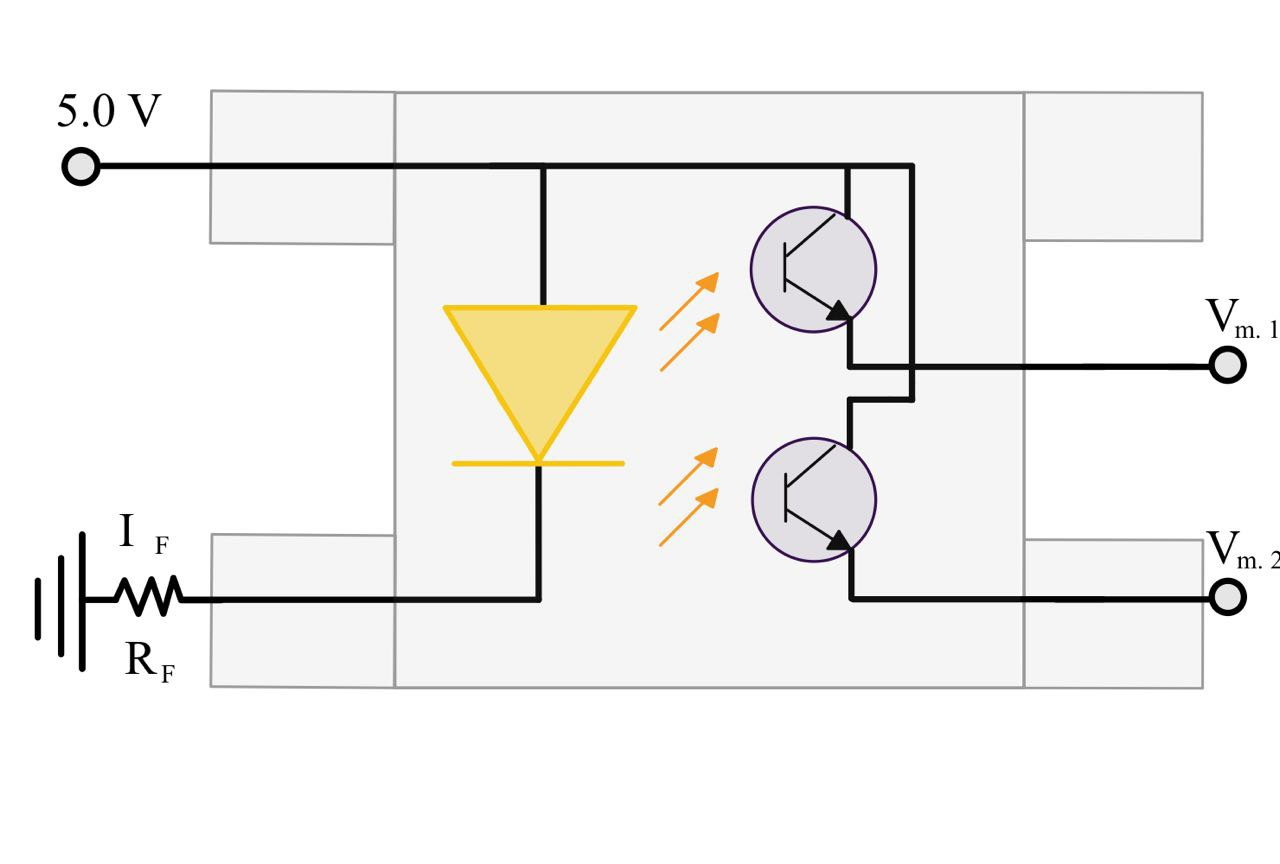
\includegraphics[width=\textwidth]{ED/dual_optopair_scheme.jpg}
    \label{fig:optopair_scheme}
    \caption{Schematic of a dual-photointerrupter sensor circuit.}
  \end{figure}

After testing the voltage measurement with oscilloscope, 
I decided to simplify the circuit presented in the research \cite{my_love_pressure_photosensor} up to the scheme \ref{fig:optopair_scheme} based on my experiments with the optopair component.
The current of the LED is limited to $I_F$ by the resistor $R_F$. %The PT maintain voltage 

\subsection{Barrier design}

Based on the provided design by the authors \cite{my_love_pressure_photosensor}, and the dimensions of the PT \ref{fig:microscopic_image}, I created the barrier and used the Finite Element Analysis in Siemens NX Software simulation to check possible force load ranges for the used geometry \ref{fig:different_materials_nx}.

\begin{figure}[H]
  \centering
  \begin{subfigure}[a]{0.4\textwidth}
    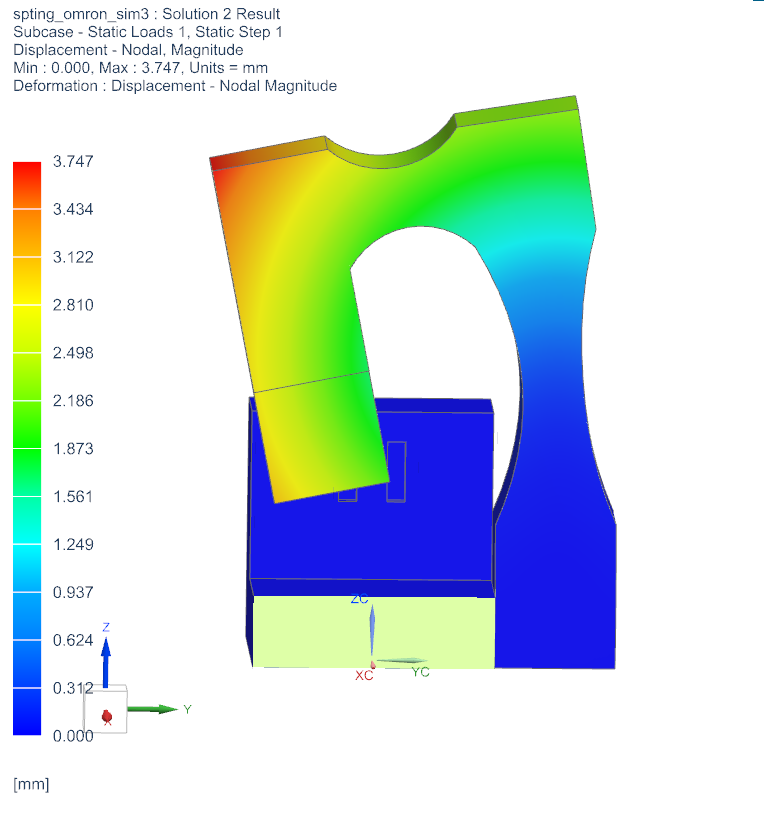
\includegraphics[width=\textwidth]{barrier_NX/Camera Roll/acrylic_10N.png}
    \label{fig:different_materials_nx:acrylic_10N}
    \caption*{(a)}
  \end{subfigure}
  \begin{subfigure}[b]{0.4\textwidth}
    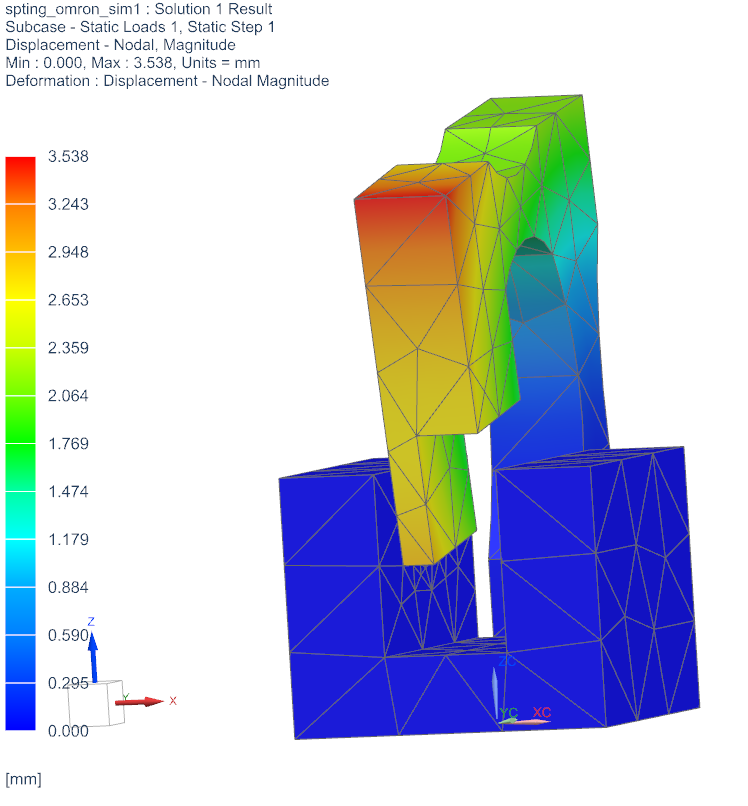
\includegraphics[width=\textwidth]{barrier_NX/Camera Roll/ABS.png}
    \label{fig:different_materials_nx:ABS}
    \caption*{(b)}
  \end{subfigure}
  
  \begin{subfigure}[c]{\textwidth}
    \begin{subfigure}[1]{0.3\textwidth}
      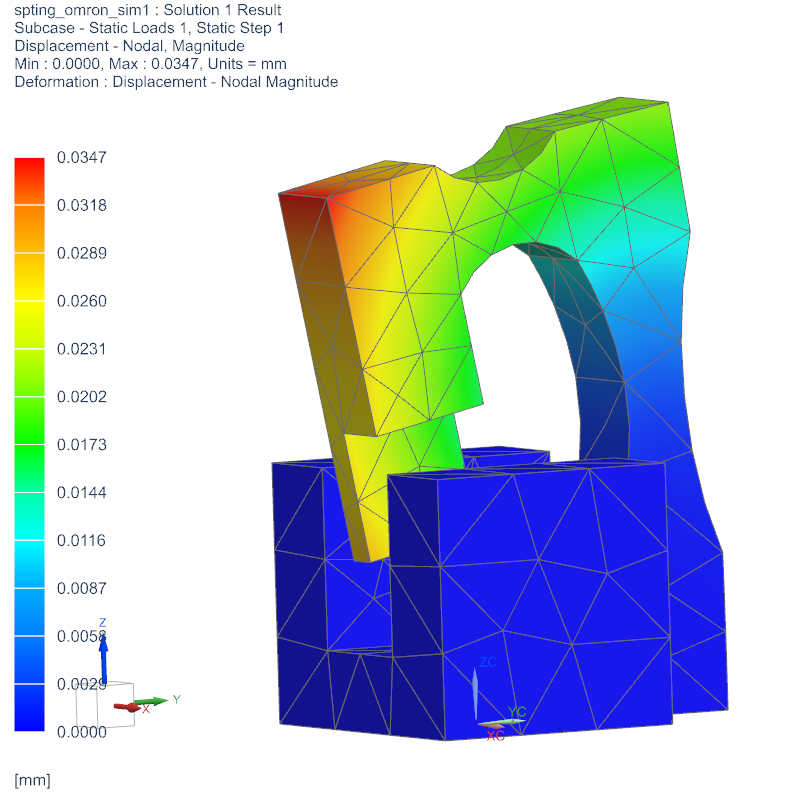
\includegraphics[width=\textwidth]{barrier_NX/Camera Roll/steel_ст3.png}
      \caption*{(1)}
    \end{subfigure}
    \begin{subfigure}[2]{0.3\textwidth}
      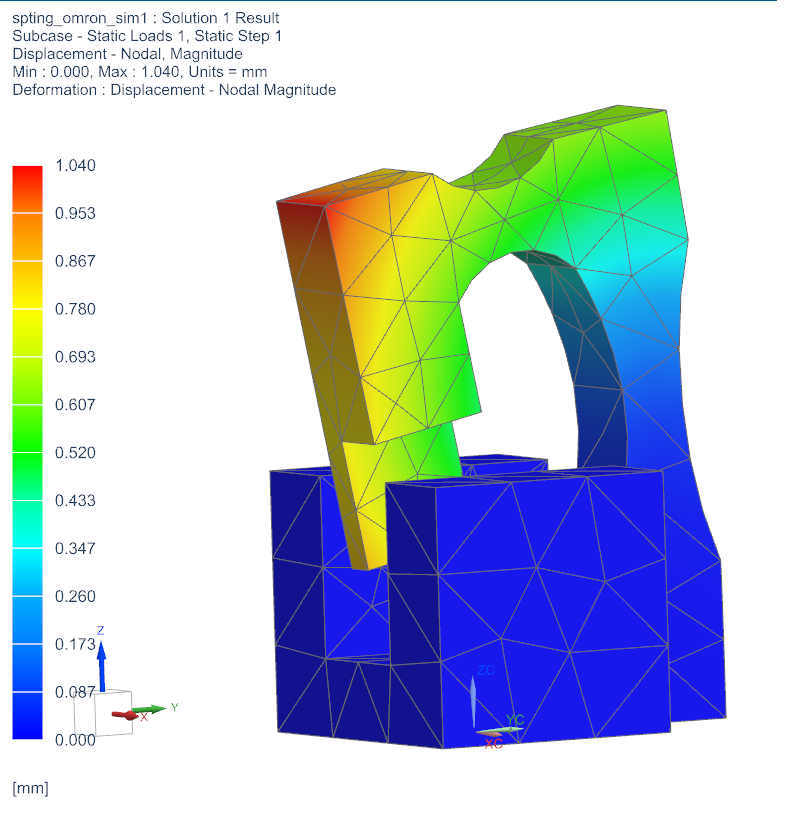
\includegraphics[width=\textwidth]{barrier_NX/Camera Roll/steel_ст3_300N.png}
      \caption*{(2)}
    \end{subfigure}
    \begin{subfigure}[3]{0.3\textwidth}
      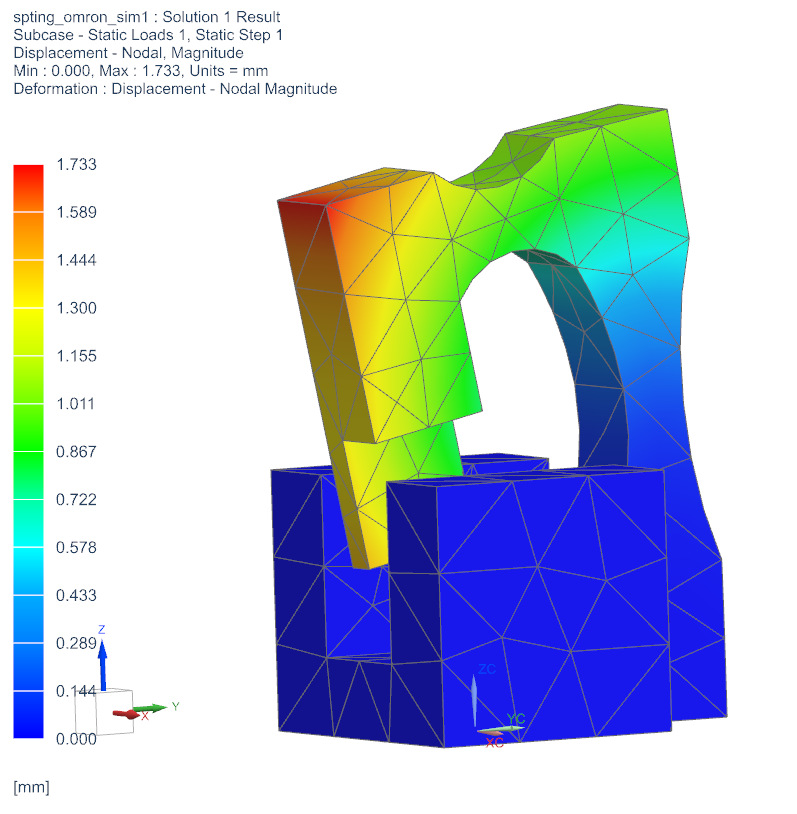
\includegraphics[width=\textwidth]{barrier_NX/Camera Roll/steel_ст3_500N.png}
      \caption*{(3)}
    \end{subfigure}
    \caption*{(c)}
    \label{fig:different_materials_nx:steel}
  \end{subfigure}
  \caption{Finite Element analysis results of the photobarrier shift from Siemens NX simulation (a) Acrylic resin 10 N, (b) ABS plastic 10 N, (c) steel with different loads: (1) 10 N, (2) 300 N, (3) 500 N}
  \label{fig:different_materials_nx}
\end{figure}

